\input{../MISC/preambule_sacado.tex}
\input{../MISC/environnements_sacado.tex}
\input{../MISC/macro_sacado.tex}
\usepackage{tkz-tab}


\title{Mathématiques 2nde  : le livre sacado}
\author{L'équipe SACADO}

\begin{document}

%\maketitle

\chapter{Fonctions de référence}{10}
{URL du parcours}
{
 \begin{CpsCol}
	\textbf{Les savoir-faire du parcours}
 	\begin{itemize}
 		\item SF1
 		\item SF2
 	\end{itemize}
 \end{CpsCol}

\begin{His}
	% Un paragraphe parlant de la vie d'un ou une mathématicien ou mathématicienne
\end{His}

\begin{ExoDec}{Compétence.}{1234}{1}{0}{0}{0}
% Un exercice de découverte/d'accroche
\end{ExoDec}
}

%%%%%%%%%%%%%%%%%%%%%%%%%%%%%%%%%%%%%%%%%%%%%%%%%%%%%%%%%%%%%%%%%%%
%%%% Page de cours 1
%%%%%%%%%%%%%%%%%%%%%%%%%%%%%%%%%%%%%%%%%%%%%%%%%%%%%%%%%%%%%%%%%%%

\begin{pageCours} % Début page de cours 1

\newgeometry{left=2cm,right=.8cm,top=1.5cm} %Ne pas toucher cette ligne

\section{La fonction Carré}

\begin{DefT}{Fonction Carré}\index{Fonctions!Carré}
La \textbf{fonction Carré} $f$ est la fonction définie sur $\mathbb{R}$ par $f(x)=x^2$.
 
La \textbf{représentation graphique} de la fonction Carré s'appelle une \textbf{parabole}\index{Parabole} et son équation est $y=x^2$. 
\end{DefT}

\begin{minipage}{0.48\linewidth}
\begin{Th} 
La fonction Carré $f$ est paire.

La parabole d'équation $y=x^2$ est symétrique par rapport à l'axe des ordonnées.
\end{Th}

\begin{ThT}{Variations de la fonction Carré}

\textcolor{red}{Démonstration exigible}

La fonction Carré est strictement décroissante sur $\mathbb{R}^-$ et strictement croissante sur $\mathbb{R}^+$. 

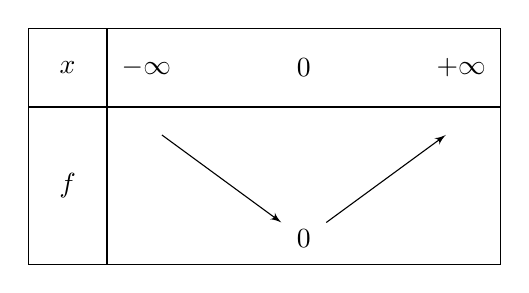
\begin{tikzpicture}
\tkzTabInit[lgt=1,espcl=2]{ $x$ / 1,$f $ / 2}
{ $-\infty$ , $0$ ,$+\infty$}
\tkzTabVar{+/$ $,-/$0$,+/$ $ }
\end{tikzpicture}

\end{ThT}



\end{minipage}
\hfill
\begin{minipage}{0.48\linewidth}

%\begin{Ill}
\definecolor{xfqqff}{rgb}{0.4980392156862745,0.,1.}
\begin{tikzpicture}[line cap=round,line join=round,>=triangle 45,x=0.7772020725388601cm,y=0.7772020725388601cm]
\begin{axis}[
x=0.7772020725388601cm,y=0.7772020725388601cm,
axis lines=middle,
ymajorgrids=true,
xmajorgrids=true,
xmin=-3.2800000000000002,
xmax=3.42,
ymin=-0.8400000000000007,
ymax=7.079999999999996,
xtick={-3.0,-2.0,...,3.0},
ytick={-0.0,1.0,...,7.0},]
\clip(-3.28,-0.84) rectangle (3.42,7.08);
\draw [color=xfqqff](1.3,1.84) node[anchor=north west] {$y=x^2$};
\draw[line width=2.pt,color=xfqqff,smooth,samples=100,domain=-3.2800000000000002:3.42] plot(\x,{(\x)*(\x)});
\begin{scriptsize}
\draw[color=xfqqff] (-2.96,8.93) node {$g$};
\end{scriptsize}
\end{axis}
\end{tikzpicture}
%%\end{Ill}

\end{minipage}

\begin{Pv}
Etude des variations de $f:x\mapsto x^2$ sur $[0;+\infty[$ :

Soient $a$ et $b$ deux nombres appartenant à $[0;+\infty[$ tels que $a<b$. 

Comparons les images de $a$ et $b$ par la fonction $f$.

$f(a)=a^2$ et $f(b)=b^2$

Pour les comparer on étudie le signe de leur différence :

$f(a)-f(b)=a^2-b^2=(a+b)(a-b)$

\begin{itemize}
\item $a$ et $b$ appartiennent à $[0;+\infty[$ donc $a+b>0$
\item $a<b$ donc $a-b<0$
\item $(a+b)(a-b)<0\Rightarrow a^2-b^2<0 \Rightarrow f(a)<f(b) \Rightarrow f(a)<f(b)$
\end{itemize}

Les images de $a$ et $b$ par la fonction $f$ sont rangés dans le même ordre que ces nombres. La fonction est donc croissante sur $[0;+\infty[$.

\end{Pv}

\section{La fonction Cube}

\begin{DefT}{Fonction Cube}\index{Inverse!Fonction}
La \textbf{fonction Cube} $f$ est la fonction définie sur $\mathbb{R}$ par $f(x)=x^3$.

\end{DefT}

\begin{minipage}{0.48\linewidth}
\begin{Th} 
La fonction Cube $f$ est impaire.

La courbe d'équation $y=x^3$ est symétrique par rapport à l'origine du repère.
\end{Th}


\begin{ThT}{Variations de la fonction Cube}

La fonction Cube est strictement  croissante sur $\mathbb{R}^-$ et strictement  croissante sur $\mathbb{R}^+$. 

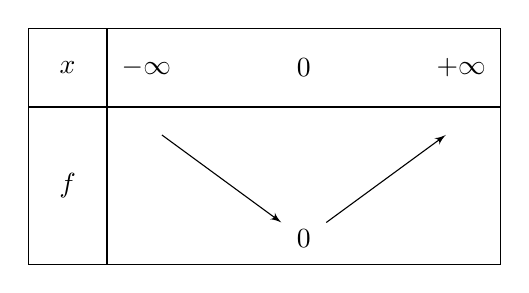
\begin{tikzpicture}
\tkzTabInit[lgt=1,espcl=2]{ $x$ / 1,$f $ / 2}
{ $-\infty$ , $0$ ,$+\infty$}
\tkzTabVar{+/$ $,-/$0$,+/$ $ }
\end{tikzpicture}

\end{ThT}

\end{minipage}
\hfill
\begin{minipage}{0.48\linewidth}

%\begin{Ill}
\definecolor{xfqqff}{rgb}{0.4980392156862745,0.,1.}
\begin{tikzpicture}[line cap=round,line join=round,>=triangle 45,x=0.7772020725388601cm,y=0.7772020725388601cm]
\begin{axis}[
x=0.7772020725388601cm,y=0.7772020725388601cm,
axis lines=middle,
ymajorgrids=true,
xmajorgrids=true,
xmin=-3.4,
xmax=3.3200000000000003,
ymin=-5.199999999999999,
ymax=5.139999999999999,
xtick={-3.0,-2.0,...,3.0},
ytick={-5.0,-4.0,...,5.0},]
\clip(-3.4,-5.2) rectangle (3.32,5.14);
\draw [color=xfqqff](1.3,1.84) node[anchor=north west] {$y=x^3$};
\draw[line width=2.pt,color=xfqqff,smooth,samples=100,domain=-3.4:3.3200000000000003] plot(\x,{(\x)*(\x)*(\x)});
\end{axis}
\end{tikzpicture}
%%\end{Ill}

\end{minipage}

\section{{Positions relatives des courbes de $x$, $x^2$ et $x^3$}}

\mini{.5\linewidth}{
\begin{Pp}
\textcolor{red}{Démonstration exigible}

\begin{itemize}
\item Si $0\leq x \leq 1$ alors $x\geq x^2 \geq x^3$.
\item Si $x\geq 1$ alors $x\leq x^2 \leq x^3$
\end{itemize}
\end{Pp}
}{.5\linewidth}{
\begin{center}
\includegraphics[width=.7\linewidth]{FIG/position_relative.png}
\end{center}
}

\begin{Pv}
Comparaison de $x$ et $x^2$ sur $[0;+\infty[$.

Pour les comparer, on étudie le signe de leur différence.

On définit la fonction $f$ par $f(x)=x^2-x$.

$f(x)=x^2-x=x(x-1)$

On peut établir le tableau de signes de $f(x)$.

$(E):f(x)=0$ alors $S(E)=\{0;1\}$\vspace{.2cm}

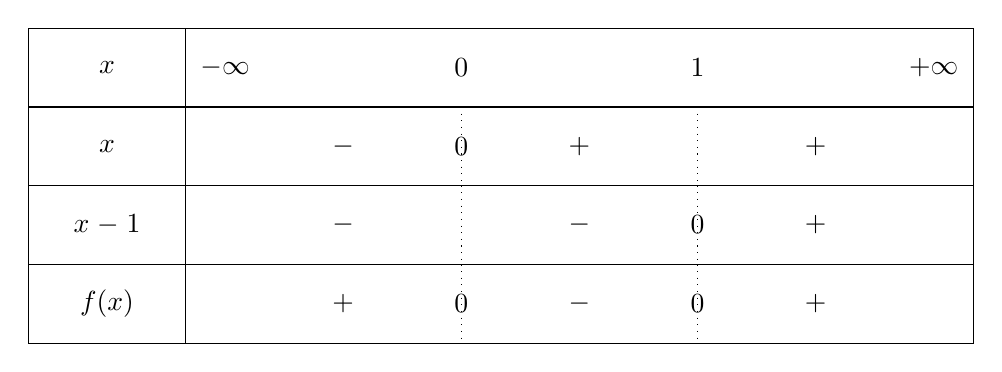
\begin{tikzpicture}
   \tkzTabInit{$x$ / 1 , $x$ / 1, $x-1$ / 1, $f(x)$ / 1}{$-\infty$, $0$, $1$, $+\infty$}
   \tkzTabLine{, -, z, +, t, +, }
   \tkzTabLine{, -, t, -, z, +, }
   \tkzTabLine{, +, z, -, z, +, }
\end{tikzpicture}

Ainsi :
\begin{itemize}
\item $\forall x \in ]0;1[,f(x)<0$ donc $x^2-x<0$ donc $x^2<x$
\item $\forall x \in ]1;+\infty,f(x)>0$ donc $x^2-x>0$ donc $x^2>x$
\end{itemize}
\end{Pv}
\end{pageCours} % Fin page de cours 1

%%%%%%%%%%%%%%%%%%%%%%%%%%%%%%%%%%%%%%%%%%%%%%%%%%%%%%%%%%%%%%%%%%%
%%%% Application direct 1
%%%%%%%%%%%%%%%%%%%%%%%%%%%%%%%%%%%%%%%%%%%%%%%%%%%%%%%%%%%%%%%%%%%

\begin{pageAD}  % Début page d'exercice d'application direct 1
\restoregeometry %Ne pas toucher cette ligne

\Sf{Connaitre et utiliser la fonction Carré}

\begin{ExoCad}{Raisonner.}{1234}{0}{0}{0}{0}{0}

Comparer sans les calculer.
\begin{description}[leftmargin=*]
\item $\left( \dfrac{3}{2} \right)^2$ et  $\pi^2$

%La fonction Carré est croissante sur $[0;+\infty]$, donc les images de deux nombres de $[0;+\infty]$ sont rangées dans le même ordre que ces nombres. Or comme $\dfrac{3}{2}<\pi$ alors $\dfrac{3}{2}^2<\pi^2$.

\point{2}

\item $(-11)^2$ et $(-6)^2$

%La fonction Carré est décroissante sur $[-\infty,0]$, donc les images de deux nombres de $[-\infty,0]$ sont rangées dans l'ordre contraire de ces nombres. Or comme $-11<-6$ alors $(-11)^2>(-6)^2$.

\point{2}

 
\item $-7^2$ et $-8^2$

%La fonction Carré est croissante sur $[0;+\infty]$, donc les images de deux nombres de $[0;+\infty]$ sont rangées dans le même ordre que ces nombres. Or comme $7<8$ alors $7^2<8^2$. Prendre l'opposé de deux nombres revient à prendre l'ordre contraire que ces nombres, ainsi : $-7^2>-8^2$.

\point{3}
\end{description}

\end{ExoCad} 


\begin{ExoCad}{Raisonner. Calculer.}{1234}{0}{0}{0}{0}{0}
\begin{itemize}[leftmargin=*]
\item Déterminer algébriquement l'intervalle de $x^2$ lorsque $x$ appartient à $[1;3]$. 

\point{2}

%La fonction $x\mapsto x^2$ est strictement croissante sur l'intervalle $[1;3]$. De plus $x$ est positif sur cet intervalle.
%
%$\textcolor{white}{\Leftrightarrow}1<x<3$
%
%$\Leftrightarrow1^2<x^2<3^2$
%
%$\Leftrightarrow1<x^2<9$
%
%Ainsi l'intervalle de $x^2$ lorsque $x$ appartient à $[1;3]$ est $[1;9]$.
\item Déterminer algébriquement l'intervalle de $x^2$ lorsque $x$ appartient à $\left[-1;4 \right]$. 

\point{3}

%La fonction $x\mapsto x^2$ est décroissante sur l'intervalle $[-1;0]$ puis croissante sur l'intervalle $[0;4]$. Traitons les deux intervalles séparément :
%
%\mini{.47\linewidth}{
%Sur $[-1;0]$, $x$ est négatif.
%
%$\textcolor{white}{\Leftrightarrow}-1<x<0$
%
%$\Leftrightarrow(-1)^2>x^2>0^2$
%
%$\Leftrightarrow1>x^2>0$
%
%Ainsi l'intervalle de $x^2$ lorsque $x$ appartient à $[-1;0]$ est $[0;1]$.
%}{.47\linewidth}{
%Sur $[0;4]$, $x$ est positif.
%
%$\textcolor{white}{\Leftrightarrow}0<x<4$
%
%$\Leftrightarrow0^2<x^2<4^2$
%
%$\Leftrightarrow0<x^2<16$
%
%Ainsi l'intervalle de $x^2$ lorsque $x$ appartient à $[0;4]$ est $[0;16]$.
%}
%
%Donc lorsque $x\in[-1,0]\cup[0,4]$, $x^2\in[0,1]\cup[0,16]$, cet intervalle peut se simplifier en $[0,16]$.

\end{itemize}

\end{ExoCad}

 
\Sf{Connaitre et utiliser la fonction Cube}

\begin{ExoCad}{Raisonner.}{1234}{0}{0}{0}{0}{0}

Comparer sans les calculer.

\begin{description}[leftmargin=*]
\item $\left(\frac{1}{5}\right)^3$ et $\pi^3$  

%La fonction cube est croissante sur $\mathbb{R}$, donc les cubes de deux nombres réels sont rangés dans le même ordre que ces nombres.
%
%On sait que $\dfrac{1}{5}=0,2$ et que $\pi\approx3$, or comme $\frac{1}{5}<\pi$ alors $\frac{1}{5}^3<\pi^3$

\point{2}

\item $(-5)^3$ et $(-9)^3$

%La fonction cube est croissante sur $\mathbb{R}$, donc les cubes de deux nombres réels sont rangés dans le même ordre que ces nombres.
%
%On sait que $-9>-5$ alors $(-9)^3<(-5)^3$.

\point{2}
\end{description}

\end{ExoCad} 

\Sf{Position relatives des courbes}

\begin{ExoCad}{Raisonner. Communiquer.}{1234}{0}{0}{0}{0}{0}

Comparer la position relative des courbes de $x^2$ et $x^3$ sur $[0;+\infty]$.

\point{5}

\end{ExoCad} 

 
\end{pageAD} % Fin page d'exercice d'application direct 1

%%%%%%%%%%%%%%%%%%%%%%%%%%%%%%%%%%%%%%%%%%%%%%%%%%%%%%%%%%%%%%%%%%%
%%%% Page de cours 2
%%%%%%%%%%%%%%%%%%%%%%%%%%%%%%%%%%%%%%%%%%%%%%%%%%%%%%%%%%%%%%%%%%%

\begin{pageCours} % Début page de cours 2

\newgeometry{left=2cm,right=.8cm,top=1.5cm} %Ne pas toucher cette ligne

\section{La fonction Inverse}



\begin{DefT}{Fonction Inverse}\index{Inverse!Fonction}
La \textbf{fonction Inverse} $f$ est la fonction définie sur $\mathbb{R}^*$ par $f(x)=\dfrac{1}{x}$.
 
La \textbf{représentation graphique} de la fonction Inverse s'appelle une \textbf{hyperbole}\index{hyperbole} et son équation est $y=\dfrac{1}{x}$. 
\end{DefT}

\begin{minipage}{0.48\linewidth}
\begin{Th} 
La fonction Inverse $f$ est impaire.

La hyperbole d'équation $y=\dfrac{1}{x}$ est symétrique par rapport à l'origine du repère.
\end{Th}


\begin{ThT}{Variations de la fonction Inverse}

\textcolor{red}{Démonstration exigible}

La fonction Carré est strictement décroissante sur $\mathbb{R}^*_-$ et strictement décroissante sur $\mathbb{R}^*_+$. 

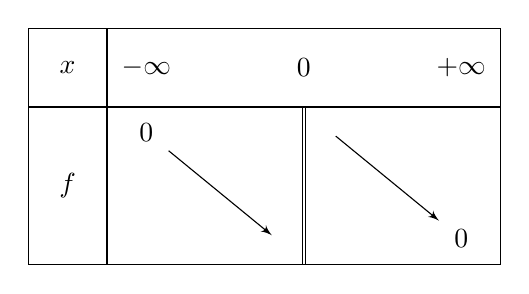
\begin{tikzpicture}
\tkzTabInit[lgt=1,espcl=2]{ $x$ / 1,$f $ / 2}
{ $-\infty$ , $0$ ,$+\infty$}
\tkzTabVar{+/$0$ , -D+ /$ $/$ $ , -/$0$}
\end{tikzpicture}

\end{ThT}

\end{minipage}
\hfill
\begin{minipage}{0.48\linewidth}

%\begin{Ill}
\definecolor{xfqqff}{rgb}{0.4980392156862745,0.,1.}
\begin{tikzpicture}[line cap=round,line join=round,>=triangle 45,x=0.7772020725388601cm,y=0.7772020725388601cm]
\begin{axis}[
x=0.7772020725388601cm,y=0.7772020725388601cm,
axis lines=middle,
ymajorgrids=true,
xmajorgrids=true,
xmin=-4.5200000000000005,
xmax=5.6000000000000005,
ymin=-4.4799999999999995,
ymax=4.499999999999999,
xtick={-4.0,-3.0,...,5.0},
ytick={-4.0,-3.0,...,4.0},]
\clip(-4.52,-4.48) rectangle (5.6,4.5);
\draw [color=xfqqff](0.62,3.38) node[anchor=north west] {$y=\dfrac{1}{x}$};
\draw[line width=2.pt,color=xfqqff,smooth,samples=100,domain=-4.5200000000000005:5.6000000000000005] plot(\x,{1/(\x)});
\end{axis}
\end{tikzpicture}
%%\end{Ill}

\end{minipage}

\begin{Pv}
Étude des variations $f:x\mapsto \frac{1}{x}$ sur $]-\infty;0[$.

Soient $a$ et $b$ deux nombres appartenant à $]-\infty;0[$ tels que $a<b$.

Comparons les images de $a$ et $b$ par la fonction $f$.

$f(a)=\frac{1}{a}$ et $f(b)=\frac{1}{b}$

Pour les comparer on étudie le signe de leur différence.

$f(a)-f(b)=\frac{1}{a}-\frac{1}{b}=\frac{b}{ab}-\frac{a}{ab}=\frac{b-a}{ab}$

\begin{itemize}
\item $a$ et $b$ appartiennent à $]-\infty;0[$ donc $ab>0$
\item $a<b$ donc $a-b<0$ donc $b-a>0$
\item $\frac{b-a}{ab}>0\Rightarrow \frac{1}{a}-\frac{1}{b}>0 \Rightarrow f(a)-f(b)>0 \Rightarrow f(a)>f(b)$
\end{itemize}

Les images de $a$ et $b$ par la fonction $f$ sont rangés dans l'ordre contraire de celui de ces nombres. La fonction inverse est donc décroissante sur $]-\infty;0[$.
\end{Pv}

\section{La fonction Racine carrée}

\begin{DefT}{Fonction Racine carrée}\index{Racine carrée!Fonction}
La \textbf{fonction Racine carrée} $f$ est la fonction définie sur $\mathbb{R}^+$ par $f(x)=\sqrt{x}$.
\end{DefT}

\begin{Rq} 
L'ensemble de définition de la fonction Racine Carrée n'est pas centré. Donc la fonction Racine carrée n'est ni paire, ni impaire.
\end{Rq}

\begin{minipage}{0.48\linewidth}



\begin{ThT}{Variations de la fonction Racine Carrée}

\textcolor{red}{Démonstration exigible}

La fonction Racine carrée est strictement croissante sur $\mathbb{R}^+$. 

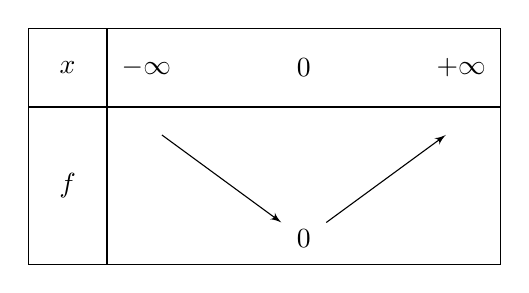
\begin{tikzpicture}
\tkzTabInit[lgt=1,espcl=2]{ $x$ / 1,$f $ / 2}
{ $-\infty$ , $0$ ,$+\infty$}
\tkzTabVar{+/$ $,-/$0$,+/$ $ }
\end{tikzpicture}

\end{ThT}

\end{minipage}
\hfill
\begin{minipage}{0.48\linewidth}

%\begin{Ill}
\definecolor{xfqqff}{rgb}{0.4980392156862745,0.,1.}
\begin{tikzpicture}[line cap=round,line join=round,>=triangle 45,x=0.7772020725388601cm,y=0.7772020725388601cm]
\begin{axis}[
x=0.7772020725388601cm,y=0.7772020725388601cm,
axis lines=middle,
ymajorgrids=true,
xmajorgrids=true,
xmin=-2.48,
xmax=7.24,
ymin=-0.78,
ymax=3.3000000000000003,
xtick={-2.0,-1.0,...,7.0},
ytick={-0.0,1.0,...,3.0},]
\clip(-2.48,-0.78) rectangle (7.24,3.3);
\draw [color=xfqqff](5.08,2.38) node[anchor=north west] {$y=\sqrt{x}$};
\draw[line width=2.pt,color=xfqqff,smooth,samples=100,domain=3.6799999990328158E-6:7.24] plot(\x,{sqrt((\x))});
\end{axis}
\end{tikzpicture}
%%\end{Ill}

\end{minipage}

\begin{Pv}
Etude des variations de $f:x\mapsto \sqrt{x}$ sur $[0;+\infty[$.

Soient $a$ et $b$ deux nombres appartenant à $[0;+\infty[$ tels que $a<b$.

Comparons les images de $a$ et $b$ par la fonction $f$.

$f(a)=\sqrt{a}$ et $f(b)=\sqrt{b}$

Pour les comparer on étudie le signe de leur différence.

$f(a)-f(b)=\sqrt{a}-\sqrt{b}=(\sqrt{a}-\sqrt{b})\times\frac{\sqrt{a}+\sqrt{b}}{\sqrt{a}+\sqrt{b}}=\frac{(\sqrt{a}-\sqrt{b})(\sqrt{a}+\sqrt{b})}{\sqrt{a}+\sqrt{b}}=\frac{\sqrt{a}^2-\sqrt{b}^2}{\sqrt{a}+\sqrt{b}}=\frac{a-b}{\sqrt{a}+\sqrt{b}}$

\begin{itemize}
\item $\sqrt{a}+\sqrt{b}>0$
\item $a<b$ donc $a-b<0$
\item $\frac{a-b}{\sqrt{a}+\sqrt{b}}<0\Rightarrow \sqrt{a}-\sqrt{b}<0 \Rightarrow f(a)-f(b)<0 \Rightarrow f(a)<f(b)$
\end{itemize}

Les images de $a$ et $b$ par la fonction $f$ sont rangés dans le même ordre que celui de ces nombres. La fonction racine carrée est donc croissante sur $[0;+\infty[$. 
\end{Pv}

\end{pageCours} % Fin page de cours 2

%%%%%%%%%%%%%%%%%%%%%%%%%%%%%%%%%%%%%%%%%%%%%%%%%%%%%%%%%%%%%%%%%%%
%%%% Application direct 2
%%%%%%%%%%%%%%%%%%%%%%%%%%%%%%%%%%%%%%%%%%%%%%%%%%%%%%%%%%%%%%%%%%%

\begin{pageAD}  % Début page d'exercice d'application direct 2
\restoregeometry %Ne pas toucher cette ligne

\Sf{Connaitre et utiliser les fonctions Inverse et Racine Carrée}



\begin{ExoCad}{Raisonner.}{1234}{0}{0}{0}{0}{0}

Comparer sans les calculer.
\begin{description}[leftmargin=*]
\item $\dfrac{1}{5}$ et $\dfrac{1}{4}$  

\point{2}

%La fonction inverse est décroissante sur $]0;+\infty[$ donc les inverses de deux nombres strictement positifs sont rangés dans l'ordre contraire de ces nombres. Or comme $5>4$ alors $\dfrac{1}{5}<\dfrac{1}{4}$.

\item $-\dfrac{1}{4}$ et $-\dfrac{1}{6}$ 

\point{3}

%La fonction inverse est décroissante sur $]-\infty,0[$ donc les inverses de deux nombres strictement négatifs sont rangés dans l'ordre contraire de ces nombres. Or comme $-4<-6$ alors $-\dfrac{1}{4}>-\dfrac{1}{6}$.

\item $\sqrt{10}$ et $\sqrt{100}$ 

%La fonction racine carrée est croissante sur $]0;+\infty[$ donc la racine carrée de deux nombres sur cet intervalle sont rangés dans le même ordre que ces nombres. Or comme $10<100$ alors $\sqrt{10}<\sqrt{100}$.

\point{2}


\end{description}

\end{ExoCad} 


\begin{ExoCadN}{Raisonner.}{0}{0}{0}{0}{0}

Expliquer pourquoi la fonction Inverse n'est pas décroissante sur $\mathbb{R}^\ast$.

 \point{3}

%Si une fonction $f$ est décroissante sur un intervalle $I$, alors pour tous nombres de cet intervalle $a$ et $b$ tel que $a<b$ on a $f(a)>f(b)$. Prenons deux nombres sur $\mathbb{R}^\ast$ et vérifions la propriété : soit $-5$ et $3$ on a $-\dfrac{1}{5}<\dfrac{1}{3}$. Ces deux nombres ne vérifie pas la propriété donc la fonction inverse n'est pas décroissante sur $\mathbb{R}^\ast$.

\end{ExoCadN}
 

 

 

\begin{ExoCad}{Représenter. Raisonner.}{1234}{0}{0}{0}{0}{0}

Résoudre graphiquement les équations, puis retrouver les résultats algébriquement.
\begin{enumerate}[leftmargin=*]
\item $\frac{1}{x}=4$ 
\point{2}

%\definecolor{ffqqqq}{rgb}{1.,0.,0.}
%\definecolor{xfqqff}{rgb}{0.4980392156862745,0.,1.}
%\begin{tikzpicture}[line cap=round,line join=round,>=triangle 45,x=1.0cm,y=1.0cm]
%\begin{axis}[
%x=1.0cm,y=1.0cm,
%axis lines=middle,
%ymajorgrids=true,
%xmajorgrids=true,
%xmin=-2.985442306278779,
%xmax=3.873024152879434,
%ymin=-1.860081495738546,
%ymax=4.998384963419662,
%xtick={-2.0,-1.0,...,3.0},
%ytick={-1.0,0.0,...,4.0},]
%\clip(-2.985442306278779,-1.860081495738546) rectangle (3.873024152879434,4.998384963419662);
%\draw[line width=2.pt,color=xfqqff,smooth,samples=100,domain=-2.985442306278779:-0.01] plot(\x,{1/(\x)});
%\draw[line width=2.pt,color=xfqqff,smooth,samples=100,domain=0.01:3.873024152879434] plot(\x,{1/(\x)});
%\draw [line width=2.pt,color=ffqqqq,domain=-2.985442306278779:3.873024152879434] plot(\x,{(--4.-0.*\x)/1.});
%\begin{scriptsize}
%\draw[color=xfqqff] (-9.206361179092708,0.06222107520861367) node {$f$};
%\draw[color=ffqqqq] (-9.206361179092708,3.868186969445704) node {$g$};
%\draw [color=black] (0.25,4.)-- ++(-2.5pt,-2.5pt) -- ++(5.0pt,5.0pt) ++(-5.0pt,0) -- ++(5.0pt,-5.0pt);
%\draw[color=black] (1.2648749360164515,4.467095308132758) node {$A(0.25, 4)$};
%\end{scriptsize}
%\end{axis}
%\end{tikzpicture}
\item $\sqrt{x}=2$ 
\point{2}

%\begin{tikzpicture}[line cap=round,line join=round,>=triangle 45,x=1.0cm,y=1.0cm]
%\begin{axis}[
%x=1.0cm,y=1.0cm,
%axis lines=middle,
%ymajorgrids=true,
%xmajorgrids=true,
%xmin=-0.5824490948339428,
%xmax=9.386811339671995,
%ymin=-0.6405197872153475,
%ymax=3.4743091840740115,
%xtick={-0.0,1.0,...,9.0},
%ytick={-0.0,1.0,...,3.0},]
%\clip(-0.5824490948339428,-0.6405197872153475) rectangle (9.386811339671995,3.4743091840740115);
%\draw[line width=2.pt,color=xfqqff,smooth,samples=100,domain=4.946052066711085E-6:9.386811339671995] plot(\x,{sqrt((\x))});
%\draw [line width=2.pt,color=ffqqqq,domain=-0.5824490948339428:9.386811339671995] plot(\x,{(--2.-0.*\x)/1.});
%\begin{scriptsize}
%\draw[color=xfqqff] (0.03644794556323789,0.20419103819161438) node {$f$};
%\draw[color=ffqqqq] (-2.5060480041765314,1.8768857419677767) node {$g$};
%\draw [color=black] (4.,2.)-- ++(-2.5pt,-2.5pt) -- ++(5.0pt,5.0pt) ++(-5.0pt,0) -- ++(5.0pt,-5.0pt);
%\draw[color=black] (4.084369128701555,2.4790558353271948) node {$B(4, 2)$};
%\end{scriptsize}
%\end{axis}
%\end{tikzpicture}
\end{enumerate}
Valider ces résultats par le calcul.

\vspace{0.4cm}

\begin{minipage}{0.48\linewidth}
\point{3}
%Pour la première équation nous trouvons graphiquement : $x=0,25$, on vérifie que $\dfrac{1}{0,25}=4$.
\end{minipage}
\hfill
\begin{minipage}{0.48\linewidth}
\point{3}
%Pour la deuxième équation nous trouvons graphiquement : $x=4$, on vérifie que $\sqrt{4}=2$.
\end{minipage}

\end{ExoCad}


\begin{ExoCad}{Raisonner. Calculer.}{1234}{0}{0}{0}{0}{0}
\begin{enumerate}[leftmargin=*]
\item Déterminer algébriquement l'intervalle de $\dfrac{1}{x}$ lorsque $x$ appartient à $[1;3]$. 

\point{3}

%La fonction inverse est strictement monotone sur $[1;3]$, l'intervalle des images sera l'image de l'intervalle à savoir $[\dfrac{1}{3};\dfrac{1}{1}]$ autrement dit $[\dfrac{1}{3};1]$.

\item Déterminer algébriquement l'intervalle de $\sqrt{x}$ lorsque $x$ appartient à $\left[1;2 \right]$. 

\point{3}

%La fonction racine carrée est strictement monotone sur $[1,2]$, l'intervalle des images sera l'image de l'intervalle à savoir $[\sqrt{1};\sqrt{2}]$ autrement dit $[1;\sqrt{2}]$.
\end{enumerate}

\end{ExoCad}
 
\end{pageAD} % Fin page d'exercice d'application direct 2

%%%%%%%%%%%%%%%%%%%%%%%%%%%%%%%%%%%%%%%%%%%%%%%%%%%%%%%%%%%%%%%%%%%
%%%% Parcours niveau 1
%%%%%%%%%%%%%%%%%%%%%%%%%%%%%%%%%%%%%%%%%%%%%%%%%%%%%%%%%%%%%%%%%%%

\begin{pageParcoursu} % Début du parcours niveau 1

%Premier exo du parcours 1
\begin{ExoCuN}{Représenter. Raisonner.}{0}{0}{0}{0}{0}
Associer à chaque représentation la fonction de référence qui lui correspond.\vspace{.2cm}

\begin{center}
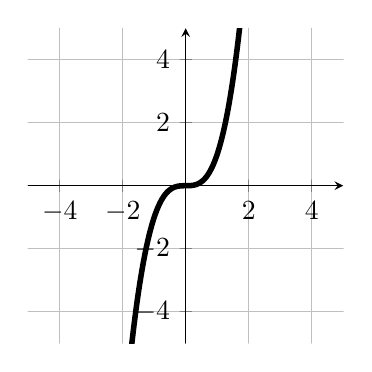
\begin{tikzpicture}[line cap=round,line join=round,>=triangle 45,x=.4cm,y=.4cm]
\begin{axis}[
x=.4cm,y=.4cm,
axis lines=middle,
ymajorgrids=true,
xmajorgrids=true,
xmin=-5,
xmax=5,
ymin=-5,
ymax=5,
xtick={-4.0,-2.0,...,4.0},
ytick={-4.0,-2.0,...,4.0},]
\clip(-5,-5) rectangle (5,5);
%\draw[line width=2.pt,smooth,samples=100,domain=-5:5] plot(\x,{(\x)^(2)});
\draw[line width=2.pt,smooth,samples=100,domain=-5:5] plot(\x,{(\x)^(3)});
%\draw[line width=2.pt,smooth,samples=100,domain=-5:5] plot(\x,{1/(\x)});
%\draw[line width=2.pt,smooth,samples=100,domain=.1:5] plot(\x,{sqrt((\x))});
\end{axis}
\end{tikzpicture}\hspace{.2cm}
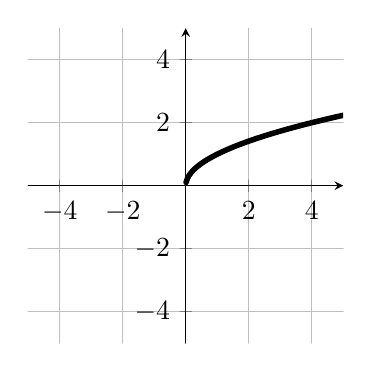
\begin{tikzpicture}[line cap=round,line join=round,>=triangle 45,x=.4cm,y=.4cm]
\begin{axis}[
x=.4cm,y=.4cm,
axis lines=middle,
ymajorgrids=true,
xmajorgrids=true,
xmin=-5,
xmax=5,
ymin=-5,
ymax=5,
xtick={-4.0,-2.0,...,4.0},
ytick={-4.0,-2.0,...,4.0},]
\clip(-5,-5) rectangle (5,5);
%\draw[line width=2.pt,smooth,samples=100,domain=-5:5] plot(\x,{(\x)^(2)});
%\draw[line width=2.pt,smooth,samples=100,domain=-5:5] plot(\x,{(\x)^(3)});
%\draw[line width=2.pt,smooth,samples=100,domain=-5:5] plot(\x,{1/(\x)});
\draw[line width=2.pt,smooth,samples=100,domain=.01:5] plot(\x,{sqrt((\x))});
\end{axis}
\end{tikzpicture}\hspace{.2cm}
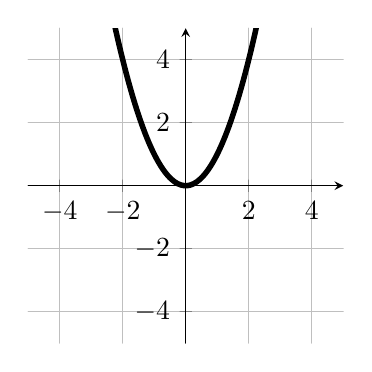
\begin{tikzpicture}[line cap=round,line join=round,>=triangle 45,x=.4cm,y=.4cm]
\begin{axis}[
x=.4cm,y=.4cm,
axis lines=middle,
ymajorgrids=true,
xmajorgrids=true,
xmin=-5,
xmax=5,
ymin=-5,
ymax=5,
xtick={-4.0,-2.0,...,4.0},
ytick={-4.0,-2.0,...,4.0},]
\clip(-5,-5) rectangle (5,5);
\draw[line width=2.pt,smooth,samples=100,domain=-5:5] plot(\x,{(\x)^(2)});
%\draw[line width=2.pt,smooth,samples=100,domain=-5:5] plot(\x,{(\x)^(3)});
%\draw[line width=2.pt,smooth,samples=100,domain=-5:5] plot(\x,{1/(\x)});
%\draw[line width=2.pt,smooth,samples=100,domain=.001:5] plot(\x,{sqrt((\x))});
\end{axis}
\end{tikzpicture}\hspace{.2cm}
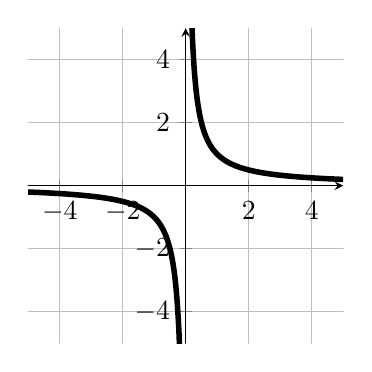
\begin{tikzpicture}[line cap=round,line join=round,>=triangle 45,x=.4cm,y=.4cm]
\begin{axis}[
x=.4cm,y=.4cm,
axis lines=middle,
ymajorgrids=true,
xmajorgrids=true,
xmin=-5,
xmax=5,
ymin=-5,
ymax=5,
xtick={-4.0,-2.0,...,4.0},
ytick={-4.0,-2.0,...,4.0},]
\clip(-5,-5) rectangle (5,5);
%\draw[line width=2.pt,smooth,samples=100,domain=-5:5] plot(\x,{(\x)^(2)});
%\draw[line width=2.pt,smooth,samples=100,domain=-5:5] plot(\x,{(\x)^(3)});
\draw[line width=2.pt,smooth,samples=100,domain=-5:-0.01] plot(\x,{1/(\x)});
\draw[line width=2.pt,smooth,samples=100,domain=0.01:5] plot(\x,{1/(\x)});
%\draw[line width=2.pt,smooth,samples=100,domain=.1:5] plot(\x,{sqrt((\x))});
\end{axis}
\end{tikzpicture}
\end{center}\vspace{.2cm}

.\dotfill
\end{ExoCuN}

%Deuxième exo du parcours 1
\begin{ExoCuN}{Raisonner. Communiquer.}{0}{0}{0}{0}{0}
Rappel : Une fonction $f$ définie sur un intervalle $I$ est dite \textbf{paire} lorsque, pour tout $x\in I$, $f(x)=f(-x)$.\\

Démontrer que $f:x\mapsto x^2$ est paire.\vspace{.2cm}

\point{3}
\end{ExoCuN}

%Troisième exo du parcours 1
\begin{ExoCuN}{Compétence.}{1}{0}{0}{0}{0}

\end{ExoCuN}

%Quatrième exo du parcours 1
\begin{ExoCuN}{Compétence.}{1}{0}{0}{0}{0}

\end{ExoCuN}

%Cinquième exo du parcours 1
\begin{ExoCuN}{Compétence.}{1}{0}{0}{0}{0}

\end{ExoCuN}

%Sixième exo du parcours 1
\begin{ExoCuN}{Compétence.}{1}{0}{0}{0}{0}

\end{ExoCuN}


\end{pageParcoursu} % Fin du parcours niveau 1
 
%%%%%%%%%%%%%%%%%%%%%%%%%%%%%%%%%%%%%%%%%%%%%%%%%%%%%%%%%%%%%%%%%%%
%%%% Parcours Niveau 2
%%%%%%%%%%%%%%%%%%%%%%%%%%%%%%%%%%%%%%%%%%%%%%%%%%%%%%%%%%%%%%%%%%%

\begin{pageParcoursd} % Début du parcours niveau 2

%Premier exo du parcours 2
\begin{ExoCdN}{Raisonner. Communiquer.}{0}{0}{0}{0}{0}

Démontrer que $f:x\mapsto x^2$ est décroissante sur $[-\infty;0[$.\vspace{.2cm}

\point{5}

\end{ExoCdN}

%Deuxième exo du parcours 2
\begin{ExoCdN}{Raisonner. Communiquer.}{0}{0}{0}{0}{0}
En utilisant la propriété de parité de la fonction $x\mapsto x^2$, montrer que $2x^2+3$ est paire.\vspace{.2cm}

\point{3}
\end{ExoCdN}

%Troisième exo du parcours 2
\begin{ExoCdN}{Compétence.}{2}{0}{0}{0}{0}

\end{ExoCdN}

%Quatrième exo du parcours 2
\begin{ExoCdN}{Compétence.}{2}{0}{0}{0}{0}

\end{ExoCdN}

%Cinquième exo du parcours 2
\begin{ExoCdN}{Compétence.}{2}{0}{0}{0}{0}

\end{ExoCdN}

%Sixième exo du parcours 2
\begin{ExoCdN}{Compétence.}{2}{0}{0}{0}{0}

\end{ExoCdN}

\end{pageParcoursd} % Fin du parcours niveau 2

%%%%%%%%%%%%%%%%%%%%%%%%%%%%%%%%%%%%%%%%%%%%%%%%%%%%%%%%%%%%%%%%%%%%
%%%%% Parcours Niveau 3
%%%%%%%%%%%%%%%%%%%%%%%%%%%%%%%%%%%%%%%%%%%%%%%%%%%%%%%%%%%%%%%%%%%%

\begin{pageParcourst} % Début du parcours niveau 3

% Premier exo du parcours 3
\begin{ExoCtN}{Compétence.}{1}{1}{0}{0}{0}
 
\end{ExoCtN}

% Deuxième exo du parcours 3
\begin{ExoCtN}{Raisonner. Communiquer.}{1}{1}{0}{0}{0}
Sachant que $a^3-a^3=(a-b)(a^2+ab+b^2)$, montrer que $f:x\mapsto x^3$ est croissante sur $[0;+\infty[$.\vspace{.2cm}

\point{5}
 
\end{ExoCtN}

% Troisième exo du parcours 3
\begin{ExoCtN}{Compétence.}{1}{1}{0}{0}{0}
 
\end{ExoCtN}

% Quatrième exo du parcours 3
\begin{ExoCtN}{Compétence.}{1}{1}{0}{0}{0}
 
\end{ExoCtN}

% Cinquième exo du parcours 3
\begin{ExoCtN}{Compétence.}{1}{1}{0}{0}{0}
 
\end{ExoCtN}

% Sixième exo du parcours 3
\begin{ExoCtN}{Compétence.}{1}{1}{0}{0}{0}
 
\end{ExoCtN}
 
\end{pageParcourst} % Fin du parcours niveau 3

%%%%%%%%%%%%%%%%%%%%%%%%%%%%%%%%%%%%%%%%%%%%%%%%%%%%%%%%%%%%%%%%%%%
%%%%  Autoevaluation/exos ouverts
%%%%%%%%%%%%%%%%%%%%%%%%%%%%%%%%%%%%%%%%%%%%%%%%%%%%%%%%%%%%%%%%%%%

\begin{pageAuto} % Début de la page d'exos ouverts

%Premier exercice : "ce que je peux avoir en éval"
\begin{ExoAutoN}{Compétence.}{1}{0}{0}{0}{0}

\end{ExoAutoN}

%Deuxième exercice : "ce que je peux avoir en éval"
\begin{ExoAutoN}{Compétence.}{1}{0}{0}{0}{0}

\end{ExoAutoN}

%%%%%%%%%%%%%%%%%%%%%%%%%%%%%%%%%%%%%%%%%%%%%%%%%%%%%%%%%%%%%%%%%%%
%%%%%%%%%%%%%%%%%%%%%%%%%%%%%%%%%%%%%%%%%%%%%%%%%%%%%%%%%%%%%%%%%%%

%Problème ouvert
\begin{ExoAutoN}{Compétence.}{1}{0}{0}{0}{0}

\end{ExoAutoN}

\end{pageAuto} % Fin de la page d'exos ouverts

%%%%%%%%%%%%%%%%%%%%%%%%%%%%%%%%%%%%%%%%%%%%%%%%%%%%%%%%%%%%%%%%%%%
%%% Page algorithmique
%%%%%%%%%%%%%%%%%%%%%%%%%%%%%%%%%%%%%%%%%%%%%%%%%%%%%%%%%%%%%%%%%%%

\begin{pageAlgo} % Début de la page d'exos d'algorithmique

%Exercice d'algorithmique
\begin{ExoAlgoN}{Compétence.}{1}{0}{0}{0}{0}

\end{ExoAlgoN}

%Exercice d'algorithmique
\begin{ExoAlgo}{Compétence.}{1}{0}{0}{0}{0}

\end{ExoAlgo}

\end{pageAlgo} % Fin de la page d'exos d'algorithmique

%%%%%%%%%%%%%%%%%%%%%%%%%%%%%%%%%%%%%%%%%%%%%%%%%%%%%%%%%%%%%%%%%%%
%%%%  Page(s) blanche(s)
%%%%%%%%%%%%%%%%%%%%%%%%%%%%%%%%%%%%%%%%%%%%%%%%%%%%%%%%%%%%%%%%%%%

\begin{pageBrouillon}

\end{pageBrouillon}

\end{document}
